\chapter{Implementation Details}
\label{chap: implementation}

This chapter covers the steps outlined in chapter~\ref{chap: emu_outline} in
significantly greater technical detail. We will name functions with which the
reader will need to be familiar in order to train an accurate emulator with
CL, as well as their limitations and the assumptions they make about their
inputs. Therefore, this chapter contains information necessary even if the
reader is interested only in using and not in modifying CL.

CL may be installed in the fashion typical of Python packages: after cloning
the repository\footnote{https://github.com/3276908917/Master}
or downloading and unzipping it, the command

\verb|pip install -e .|

should be run in the top-level directory (``Master'') and in the
appropriate environment (when using a package manager such as Anaconda).
The reader should keep in mind that we refer to the package as CL in this
thesis to clearly distinguish it from the Boltzmann solver CLASS, but its
true name (for example, for use in \texttt{import} statements) is
\texttt{cassL}.

\section{Building the Latin Hypercube}
\label{sec: build_lhc}

% lhc.py

In this section, we will discuss the building of LHSs, which within CL is 
handled by \texttt|lhs|. As mentioned in section~\ref{sec: lhc_outline},
we first create a unit LHS and then later rescale it according to a set of
priors.

Each entry $\bm{x}$ in our LHS $\matr{X}$ will be either a four- or
six-dimensional vector, 
depending on the emulator's support for massive neutrinos. When building a
massless-neutrino emulator, each $\bm{x}$ will describe the $\omega_b$,
$\omega_c$, $n_s$, and
$\tilde{\sigma}_{12}$ values for a different cosmology in 
this order. When building a massive-neutrino emulator, each $\bm{x}$ will 
additionally specify the $A_s$ and $\omega_\nu$ values for that cosmology, 
again in this order.

To get started generating LHSs, we integrated demonstration code written by 
Daniel Farrow \textcolor{orange}{(and who else?) add these people to the 
Danksagung}. We begin by invoking the \texttt{lhs} function of
\texttt{pyDOE2} a number of times. Each time we get a random new unit LHC, 
whose spacing we analyze with the \texttt{cdist} function from
\texttt{scipy.spatial.distance}.
Recall from section~\ref{sec: lhc_theory} that
our samples more evenly cover the sample space if the minimum separation
$s^*$ increases. Therefore, from among the numerous calls of \texttt{lhs} we 
select the LHS with the largest minimum separation.

In order to maximize the number of random hypercubes generated per unit of
wall time, we have written a multithreaded function called
\verb|multithread_unit_LHC_builder| \textcolor{orange}{Keep your eye on this
one, I'm thinking about condensing lhc.py to just a couple of functions.}
Through the function parameter \verb|num_workers| the user is free to assign
any number of CPU threads to the task; in principle, a CPU can be
wholly dedicated to the optimization of the LHS.
\verb|multithread_unit_LHC_builder| does not contain a return statement but
instead triggers an unending query for LHSs. The user is notified via command
line printout whenever an LHS has been generated whose $s^*$ exceeds
the previous record. Whenever such a superior LHS is
encountered, the function writes the LHS to a file and continues. Therefore,
the user may run this script in the background and terminate whenever. The
function always writes LHSs to the same file, so each new record-setting LHS
overwrites the old one. When the user terminates the function, whatever output
file remains represents the best LHS seen since the function was first called.

%%% It's just too much detail for a master's thesis, no one will care
\begin{comment}
The \verb|cdist| function can be re-used to compare LHSs loaded from 
different
files. However, since there is generally little reason to keep old LHSs
(except, perhaps, to reconstruct specific emulators), it reduces clutter to
simply continue overwriting the same file. Therefore, the function
\verb|multithread_unit_LHC_builder| also includes a parameter
\verb|previous_record|, which is recommended whenever the user would like to
stop the function and then resume it later. In such a case, the parameter
should be set to the \verb|cdist| value of the exis}
\end{comment}
%%%

% I've got a better idea: the function should automatically ask the user if
% he's sure, in the case that we find a file under the name under which we
% intend to write. If the user is sure, we take the cdist of that existing
% file and use it as the previous record!

% we multithreaded the Python script to spawn 12 workers on an 11th gen Intel 
% i7-11700 @ 2.50 GHz. IF YOU ARE USING THE WORK DESKTOP

As of 2 October 2023, CL relies on this brute-force approach to build the
LHSs that are eventually used to train the emulators. To understand the 
computational and wall-time costs associated with this solution, we include 
plots~\ref{fig: function_calls} and~\ref{fig: wall_time}.

% The following plots were generated with h_units_bad.ipynb
\begin{figure}[ht!]
    \begin{subfigure}{0.45 \textwidth}
    \centering
 		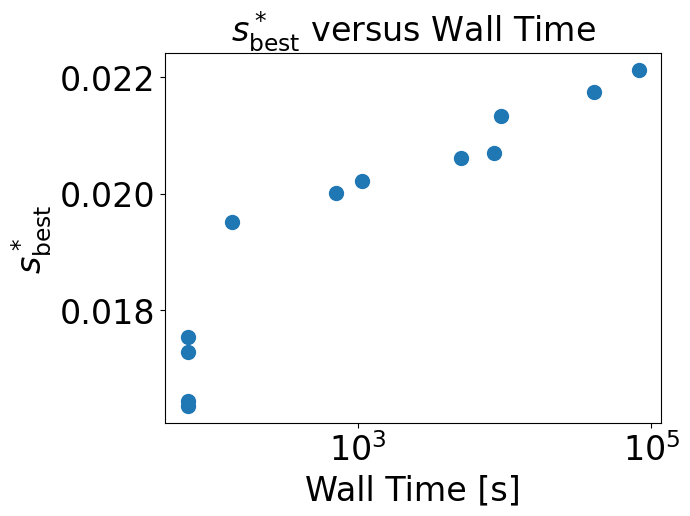
\includegraphics[width=\textwidth]{wall_time}
 		\caption{Using $h$ units.}
 		\label{fig: wall_time}
    \end{subfigure}
    \begin{subfigure}{0.45 \textwidth}
    \centering
 		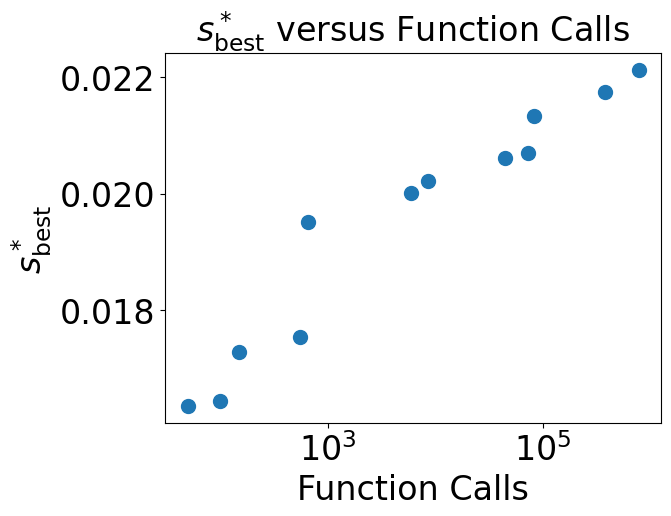
\includegraphics[width=\textwidth]{fn_calls}
 		\caption{Using absolute units.}
 		\label{fig: function_calls}
    \end{subfigure}
        \centering
    \caption[Efficiency of Brute-Force LHS Approach]
    		{It's not very good...}
    \label{fig: random_lhs_performance}
\end{figure}

\begin{comment} % The following paragraph says this stuff better
we left the system to run for two days. In this time, the 
largest minimum separation that we generated was approximately 0.08022.  
Recall from section sec_B1 that the theoretical best possible value for this 
setup is approximately 0.24183. It would have been more meaningful if you had 
counted the total number of function calls, but it isn’t too late to set up 
such a run. So, even after assigning a relatively large amount of compute to 
this brute force solution, we fail to obtain an LHC of even a third of the 
best minimum separation.
\end{comment} 

Remember from section~\ref{sec: lhc_theory} equation~\ref{eq: best_lhs_sep},
which tells us the best possible $s^*$
given dimension $d$ and total number of samples $N_s$. Let us consider a 
massless-neutrino emulator (a total of four dimensions per cosmology vector)
trained over five-thousand CAMB spectra. If we plug in $d = 4$ and $N=5000$,
we find $s^*_\text{best} \approx 0.1189$. Clearly, the brute force method
achieves only a comparatively low $s^*$, even over the span of multiple days.

Based on figures~\ref{fig: function_calls} and~\ref{fig: wall_time}, we
claim that our approach is inefficient and not well-suited to the approach of 
maximizing $s^*$. Since suboptimal $s^*$ values imply unevenness in the
coverage of the space of cosmologies, we expect low $s^*$ values to impact
the emulator by increasing variance in the errors, because the worst errors
will be significantly worse, while the best errors will be slightly better in
oversampled regions. We also expect the average error to increase slightly,
as the oversampled regions should benefit less than the undersampled regions
suffer.

% One could argue that the variance in oversampled regions will decrease to
% compensate, right? I need to clarify that the decrease in variance in the
% oversampled regions would not be able to compensate the increased variance
% in the undersampled regions, because the space of power spectra is
% continuous, so closely spaced points reveal less about the true function
% than well spaced points.

We will test these expectations in section~\ref{sec: error_from_lhc} by
varying the $s^*$ of the LHS with which we train the emulator.
\textcolor{orange}{We will explore the question of superior methods in
section~\ref{sec: future_work}}.

\section{Rescaling the LHS}
\label{sec: lhc_rescale}

%s Introduce the build_cosmology script

Now that we have a unit LHS $\matr{X}_u$, we need to scale it 
so that each axis, which currently runs from zero to one, runs along a range 
dictated by one of the priors. This scaling is handled by the \texttt{ged}
function \verb|build_cosmology|. It accepts as parameters the values of
$\omega_b$, $\omega_c$, $n_s$, $\sigma_{12}$, $A_s$, $\omega_\nu$, and, 
optionally, a dictionary of priors. If this
dictionary is not provided, the cosmological parameters are assumed to
already have been scaled. When building a massless-neutrino emulator,
the information $\omega_\nu = 0$ and $A_s = A_s(\text{Aletheia model 0})$ is
automatically provided to \verb|build_cosmology| by
\verb|fill_hypercube|. 
% We really should redo build_cosmology so that it assumes indices match to
% the same parameters every time! This is how the rest of the code works,
% after all.

The precise form of the scaling is given by the formula for transforming a
random variable $x \sim \mathcal{U}(0, 1)$ to a random variable
$x' \sim \mathcal{U}(a, b)$:

\begin{equation}
\label{eq: scaling}
x' = x (b - a) + a
\end{equation}

After scaling the parameters, \verb|build_cosmology| finishes bridging the gap
between the LHS and the CAMB \verb|pars| object (as introduced in
chapter~\ref{chap: CAMB_setup}) by using default values to fill in the
remaining values demanded by CAMB. For example, $H_0$, $w_a$ and $w_0$ are
not parameters over
which we train the emulator, but CAMB requires that they be specified before
a power spectrum can be calculated. In all such cases, we use Aletheia model
0 as default values. \textcolor{orange}{I'm not referring to table 1.2 here
because I would have to expand it with parameters not essential to this work,
so I would have to redo the captions for fig 1.1 and table 1.2...}

So long as the power spectrum's value for $\sigma_{12}$ agrees with the
prior-scaled value from the LHS, it should not matter that 
we use the model 0 values, as these are evolution parameters.
\textcolor{red}{Or should it? If this logic really held, shouldn't we be able 
to modify $w_a$ and $w_0$ in order to get the correct value of
$\tilde{\sigma}_{12}$? But these are evolution parameters, so why don't we?}

\section{Integrating Evolution Mapping}
\label{sec: generate_emu_data}

% generate\_emu\_data.py

%s Now talk about fill_hypercube, a central function of this script

\verb|fill_hypercube| is the central function of \texttt{ged}. It iterates 
through the rows $\bm{x}$ of the unit LHS
$\matr{X}_u$, packages them into a fully-specified cosmology using
\verb|build_cosmology|, and passes the cosmology to one of the 
evaluation functions. \texttt{ged} provides two evaluation functions, which 
combine the CAMB calls from \texttt{ci} with the
principles of evolution mapping: \verb|direct_eval_cell| relies on
\verb|evaluate_cosmology| while \verb|interpolate_cell| relies on
\verb|cosmology_to_Pk_interpolator|. These two options are designed to give
the same results and will differ at a level insignificant to the conclusions
of this work. The emulator pipeline uses the direct evaluation approach by
default.

%s What exactly does it mean here to integrate evolution mapping into the 
%s code?

Recall from chapter~\ref{chap: CAMB_setup} that CAMB does not accept
$\sigma_{12}$ as an input. The importance of \verb|direct_eval_cell| and 
\verb|interpolate_cell| is in circumventing this problem.
After \verb|build_cosmology| returns a complete cosmology dictionary, these
functions computer the MEMNeC. Then, they request CAMB power spectra for the
MEMNeCs at 150\footnote{150 is the maximum number of redshifts that CAMB will
accept in a single call.} linearly-spaced redshifts in the
interval [0, 10]. \textcolor{orange}{log spacing would have been better for
redshift}. This interval suffices to capture the reddest galaxies
in our galaxy redshift surveys. \textcolor{green}{citation}. Next, these
functions request a one-dimensional interpolator from \texttt{scipy} with
the $\tilde{\sigma}_{12}$ values as the $x$ and the $z$ values as the $y$.
By passing the desired $\tilde{\sigma}_{12}$ value to the interpolator, we
can in principle find the redshift at which we need to call CAMB.

%s Bonus section that doesn't really fit anywhere specific: speed-up

Since we are estimating this redshift from an interpolation over 150 power
spectrum samples, the $z_\text{interp}$ returned by our interpolator does not
\textit{exactly} match the theoretical $z_\text{exact}$ at which the
power spectrum would exactly match the desired input value,
$\tilde{\sigma}_{12}(z_\text{exact})$. In order to speed up \texttt{ged},
which is by far the most time-intensive step in the emulator pipeline,
\verb|direct_eval_cell| and \verb|interpolate_cell| stop at one iteration of 
interpolation and return $\tilde{\sigma}_{12}(z_\text{interp})$. Then,
\verb|fill_hypercube| mutates the $\tilde{\sigma}_{12}$ column of the original 
LHS by using the reverse transformation of~\ref{eq: scaling}:

\begin{equation}
x = \frac{x' - a}{b - a}
\end{equation}

to obtain the unit counterpart to $\tilde{\sigma}_{12}(z_\text{interp})$.
This transformed value replaces the original value found in the LHS.
Once \verb|fill_hypercube| finishes computing the spectra, the user
should save the LHS to a new file (marked ``final'' in
figure~\ref{fig: flow_chart}); this LHS is used in the emulator's training.

This shortcut saves a good deal of time but moves the value of
$\tilde{\sigma}_{12}$ negligibly
\textcolor{green}{cite some numbers for this claim!}.
The only downside of moving $\tilde{\sigma}_{12}$ could be that it
decreases the $s^*$ of the LHS. Since the value shifts only weakly, we do not
consider it to produce a relevant decrease in the accuracy of the emulator.

\textcolor{orange}{We should make error plots (comparing the two approaches 
with hyper cube as a control), but I strongly suspect the error will be 
negligible.}

In theory, the above procedure suffices to match any $\tilde{\sigma}_{12}$
value. However, for some cosmologies, $z_\text{exact} < 0$, a case not
currently supported by CAMB. Since all power spectra grow in amplitude with
time, we can quickly establish whether the cosmology is ``solvable'' by
verifying that

\begin{equation}
\label{eq: solvability_cond}
\tilde{\sigma}_{12}(z = 0) \geq \tilde{\sigma}_{12}(z_\text{exact})
.\end{equation}

When this condition is not fulfilled, we can modify the value of $h$ to
compensate. Recall from chapter~\ref{chap: A_s} that changing $h$ while
holding $\omega_b$, $\omega_c$, and $\omega_K$ fixed amounts to varying
$\omega_\text{DE}$, an evolution parameter. Since $h$ is an evolution
parameter in this context, we are free to modify it in order to increase the
range of solvable cosmologies. Although CAMB nominally accepts $h$ values as
low as 0.01, in practice we find that values below around
$h_\text{min} \approx 0.07$ sometimes lead to crashes.

We call this process of tweaking the $h$ and $z$ values
`\textit{re}scaling' to
succinctly distinguish it from the application of priors to scale a unit LHS.
In chapter~\ref{chap: emu_outline}, we noted that \texttt{ged} outputs
files containing rescale parameters. These files contain the $(h, z)$ pairs
at which we evaluated each cosmology in the input LHS. Since we train our
emulator over neither $h$ nor $z$, this information is inconsequential to the
construction and testing of the emulator. Instead, these files are useful for
independently verifying the accuracy of the pipeline.

Unfortunately, even when setting the dimensionless Hubble parameter to its
minimum safe value, some power spectra will still fail
condition~\ref{eq: solvability_cond}.
For the purposes of this treatment, we refer to such cosmologies as
``unsolvable.'' An emulator can still be trained even if only one of the input 
cosmologies is solvable. However, the occurrence of even one
unsolvable cosmology indicates that the actual range of parameters in the
training data is narrower than the nominal input priors. 

The problem of unsolvable cosmologies led us to create the
increasingly restrictive prior sets described in
section~\ref{sec: lhc_outline}.
Of the three provided pairs of priors files, only the COMET priors
(table~\ref{tab: COMET_priors}) are narrow enough to completely evade the 
issue of unsolvable cosmologies. For this reason, the COMET priors are the
defaults used by CL. We defer further discussion of unsolvable cells to
section~\ref{sec: prior_woes}.

%s Don't give up skeleton!


\section{Training the Emulator}
\label{sec: train_emu}

% train\_emu.py

Once \texttt{ged}'s \verb|fill_hypercube| completes, the user is ready to
begin training the emulator. We recommend that the user store all of the
relevant data files in a subdirectory of \verb|data_sets|, which is a
subdirectory of the \texttt{cassL} code directory. This organization
allows the user to load and repackage all of the essential data with the
\texttt{ui} function \verb|get_data_dict|, which returns the
``data dictionary'' represented in figure~\ref{fig: flow_chart}.
Once the user passes the data dictionary to the \texttt{ui} function
\verb|build_and_test_emulator|, the end of the emulator pipeline has been 
reached, and the remaining work is automatic.

First, \verb|build_and_test_emulator| cleans the input data by dropping
unsolved cosmologies from the training and testing sets. Next, to train a new 
emulator, \\
\verb|build_and_test_emulator| instantiates the
\verb|Emulator_Trainer| class. We refer to such objects as \textit{trainers}.
Each emulator is an instance of
the \texttt{Emulator} class with a \texttt{GPy}
\texttt{GPRegression} object at its core. We 
refer to instances of the \texttt{Emulator} class as \textit{emulator 
objects}.

The GPR object is the core of the emulator and handles the training
and prediction. An extremely simple setup for training a GPR object
\texttt{gpr} would consist of the following four lines:

\begin{verbatim}
kernel = GPy.ker.RBF(input_dim=6, variance=1., lengthscale=1.)
gpr = GPy.models.GPRegression(X_train, Y_train, kernel)
gpr.constrain_positive('')
gpr.optimize()
\end{verbatim}

\textcolor{red}{Does it make any sense to put a comma after the code listing?}

where `' in the second line is a regex matching all parameter names. This
example of course assumes a massive-neutrino setup, as the kernel dimension is
six. The true kernel used by CL is more complicated. After experimenting with
different options, we find that combining the RBF, Mat\'{e}rn, and white noise
kernels leads to the best results.

The primary purpose of \texttt{Emulator} is to simplify access to the
\texttt{GPRegression} object. The \texttt{GPRegression} object is trained on
normalized $\matr{X}$ and $\matr{Y}$ data, and therefore outputs normalized
predictions. The emulator object will automatically convert input cosmologies
to a normalized format and output power spectra to a denormalized format.

Normalization involves transforming the $\matr{X}$ and $\matr{Y}$ data sets
away from extreme values, optimally toward a [0, 1] interval.
Normalization represents a crucial step in the emulation pipeline,
as it makes a significant difference in accuracy. For example, the difference
between an emulator with $\matr{Y}$ normalized and an emulator with
both $\matr{X}$ and $\matr{Y}$ normalized can be an order of magnitude in the
dynamic range of the error curves. 

The $\matr{Y}$ normalization is by far the more important. As seen in
figure~\ref{fig: first_power_spectrum}, the power spectrum spans a over five
orders of magnitude. In order to decrease both the overall magnitude as well
as the dynamic range, we apply the following transformation:

\begin{equation}
\label{eq: y_normalization}
y'_i = \frac{\ln{y_i} - \bar{y}_i}{\sigma_{y_i}}
,\end{equation}

where the $i$ subscripts indicate the index of the $k$-bin; $y'$ is the 
normalized spectrum; $\bar{y}_i$ is the average over all
$\bm{y} \in \matr{Y}$; and $\sigma_{y_i}$ is the 
standard deviation over all $\bm{y} \in \matr{Y}$.

By contrast, as long as we keep the priors separate from the unit LHS, we can
simply use $\matr{X}_u$ as our training data. This explains why we
maintain the priors and LHSs as separate entities throughout the entire
pipeline, and only ever combine them temporarily, such as during the
calculation of the CAMB spectra. 

The need for normalization transcends more mundane numerical instabilities
like overflow and underflow. For example, even if a parameter's 
prior range falls within the relatively reasonable [0.0001, 0.0006] interval, 
its emulation will still be improved by normalizing the parameter to a [0, 1] 
interval. Nonetheless, the improvement will be more dramatic the further away 
a prior is from this [0, 1] interval.

Consider the prior in $A_s$, which 
regardless of the choice between the three default priors files, covers 
extremely small values (on the order of $10^{-9}$). Without the appropriate 
normalization, the trained GPR will be nearly insensitive to the impact of 
$A_s$. Since $A_s$ is essential to capturing the effect of $\omega_\nu$,
the emulator behaves similarly to a massless-neutrino emulator, and the lack 
of neutrino dependence dominates the error.

\textcolor{orange}{Can we add some material in
section~\ref{sec: gpr_intro}: why is GPR vulnerable in this way?}

\textcolor{orange}{Briefly explain what GPy is doing--don’t treat it like some 
black box.}


\section{Accessing and Using the Emulator}

The user can initialize a new trainer either by
passing in a file name associated with a pickled emulator object or by
calling the constructor with the name, $\matr{X}_{u, \text{train}}$,
$\matr{Y}_\text{train}$, and priors of the emulator. The trainer will assume
that the $\matr{X}$ data are already normalized, so remember to keep the unit
LHS separate from the priors. By contrast, the trainer assumes that the
$\matr{Y}$ are not yet normalized. It automatically computes and stores
$\bar{\bm{y}}$ and $\bm{\sigma}_y$, and then computes
transformation~\ref{eq: y_normalization}.
The $\bar{\bm{y}}$ and $\bm{\sigma}_y$ are determined exclusively by the
training data and are therefore constants.

To make a prediction with the newly trained emulator object, the user must
first define a cosmology in the form of an array with the same dimension as 
the training points: four for the massless-neutrino case, six for the
massive-neutrino case. The array must be normalized, for which purpose the
emulator object's \verb|convert_to_normalized_params| function exists:
given some non-normalized cosmology array, the emulator object will apply its
priors to map the values to the same [0, 1] intervals over which the
\texttt{GPRegression} object was trained.

Once the input cosmology is normalized, the user can obtain the power
spectrum by calling the emulator object's \verb|predict_pspectrum| function.
This function automatically denormalizes the prediction according to the
stored $\bar{\bm{y}}$ and $\bm{\sigma}_y$ arrays by applying the inverse
transformation of~\ref{eq: y_normalization}:

\begin{equation}
y_i = \exp (\sigma_{y_i} y'_i + \bar{y}_i)
\end{equation}


\section{Testing the Emulator}
\label{test_emu}

The majority of the quantification and visualization of the performance of the
emulator are left to the user. However, a couple of functions are provided for 
the sake of simple ``eyeball'' evaluation of the emulator's accuracy.
The trainer's \texttt{test} function takes a set of $\matr{X}$ and $\matr{Y}$ 
test data and computes errors automatically. As in the trainer's constructor,
the $\matr{X}_u$ should be the \textit{unit} LHS for the training data, and
therefore already normalized. In the same manner, the $\matr{Y}$ should not
already be normalized.

The \texttt{test} function stores three sets of error 
metrics as class attributes for the trainer: \texttt{deltas[i][j]}
is the simple difference between the $i$-th predicted spectrum and the
$i$-th test spectrum in the $j$-th $k$-bin;
\verb|rel_errors[i][j]| is the ratio of \texttt{deltas[i][j]} to the
value of the $i$-th test spectrum in the $j$-th $k$-bin; and
\verb|sq_errors[i][j]| is the square of \texttt{deltas[i][j]}).
It follows from the definition of these error metrics that all of them have 
the same dimensions as $\matr{Y}_\text{test}$.
\textcolor{orange}{In the current
version of the code, this number of scales must be equal in the training and
testing sets. But, if we add another layer of interpolation, we could easily
eliminate this limitation}.

The \verb|error_curves| function graphs the performance on the given test set 
using a collection of overplotted error curves, where each curve represents a 
single cosmology. By default, the $y$-axis is relative error and the
$x$-axis is the inverse scale, $k$. To break down the performance based on 
individual cosmological parameters, there is a \verb|param_index| function
parameter which will automatically color each curve according to its value in 
the chosen cosmological parameter. Since colors can sometimes be difficult to 
quickly compare, there is also a \verb|fixed_k| function parameter. When a 
fixed value for $k$ is provided, the output is a scatter 
plot, with percent error as the $y$-axis and the chosen cosmological parameter 
as the $x$-axis.

The \verb|error_statistics| function issues a rudimentary summary of the 
application of some NumPy aggregator\footnote{The user may also pass in
non-NumPy aggregators as long as they can be called in the exact same
way--the \verb|error_statistics| and \verb|error_hist| functions always
perform the call \verb|error_aggregator(errors, axis=1)|.}
\verb|error_aggregator|, which condenses each error array to a single point,
to one of the various error metrics described earlier. The 
most useful aggregators will be \verb|mean|, \verb|median|, and \verb|std|, 
but interesting information can also be gathered from, for example, the
\verb|min|, \verb|max|, and \verb|ptp| aggregators.
\verb|error_statistics| simply prints various statistics associated with the 
aggregation, such as the median of the aggregates.

The \verb|error_hist| function is essentially a visualization of the 
information printed out by the \verb|error_statistics| function: an aggregator
function is applied to the selected error array, then the aggregates are 
binned and plotted as a histogram. The user can specify the number of bins,
otherwise Sturges' rule is used.

\textcolor{orange}{Where are the training errors?}

These testing functions are important to understand because their results
drive the appraisals of the various emulators produced and discussed in
chapters~\ref{chap: default_emu} and~\ref{chap: disc_and_conc}. Now that we
have covered all of the essential steps in building an emulator, we are
prepared to investigate its accuracy. We begin in
chapter~\ref{chap: default_emu} by concentrating on a simple case: the
default emulators CL will build.
